\section{Feedback impl.}

\frame{

After several experiments came to this scheme with the summing amplifier:
\begin{center}
    \incfig{scheme3}
\end{center}

Photodiode power is enough to not use an additional amplifier. \frametitle{Scheme}}

% вставить слайд с вахами и картинками:
% хватает усилиения, 

% \frame{
% 
Makes sense to be in the most sensitive range, it was measured: \\
 -\ $I$-$V$ curve  for a laser \\
 -\ the dependence of the ph. diode voltage on the laser power.

\begin{figure}[h]
    % \centering
    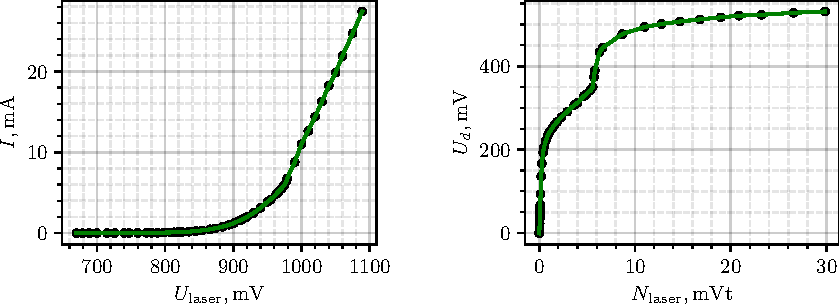
\includegraphics[width=1.0\textwidth]{figures/IV.pdf}
    %\caption{}
    %\label{fig:}
\end{figure}

So, laser voltage range of  $0.85$V selected. \frametitle{I–V curve}}

\frame{

Makes sense to be in the most sensitive range, it was measured: \\
 -\ $I$-$V$ curve  for a laser \\
 -\ the dependence of the ph. diode voltage on the laser power.

\begin{figure}[h]
    % \centering
    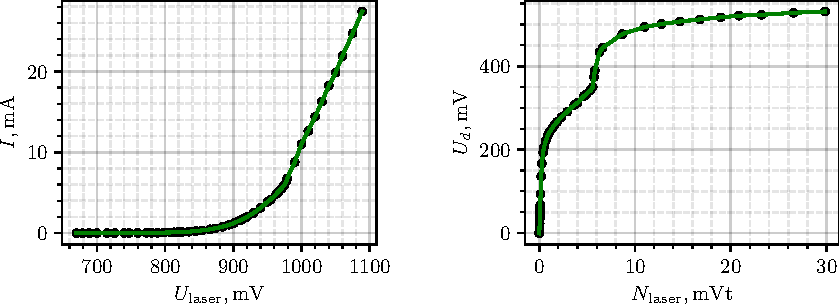
\includegraphics[width=1.0\textwidth]{figures/IV.pdf}
    %\caption{}
    %\label{fig:}
\end{figure}

So, laser voltage range of  $0.85$V selected. \frametitle{I–V curve}}

\frame{
For testing, the assembly was carried out on the dumping board.
\begin{center}
    \incfig{scheme4}
\end{center}

\hspace{-3mm}
\textbf{Thus, a scheme with positive feedback was implemented.} \\

\hspace{-3mm}
However, no desired oscillations were observed. \frametitle{Realization}}

% варьируя длина оптоволокна -- можем контролировать
% то что нашли -- маломощное, подходя к нужным мощностям всё же сжигали.
% научились стабилизировать оу, поняли необходимость аккура
% 
\frame{
With used amplifiers, the following oscillations at the amplifier output with DC power can be observed:

\begin{center}
    \incfig{scheme5}
\end{center}

This is due to the instability of the amplifier. 
% This instability can be eliminated by the adjustment of the scheme. 

\phantom{42}

The main problem is that desired oscillations $\sim 10$ ns. \\

\phantom{42}

We proceeded to experiments with faster amplifiers, but it is usefull to understand results of such delays.

oscillations megahertz
 \frametitle{Problems}}

% \frame{
% However, it was not possible to move to the chaotic regime in the laser. Possible cause of the problem may be
\begin{itemize}
    \iitem{parasitic capacity and inductance,}
\end{itemize}
In terms of solutions -- neatly soldered scheme.


% \phantom{42}

% A suitable amplifier, with similar properties used in the article, must come in June. \frametitle{Problems}}


\frame{
In real system\footnote{
    S. Tang, J. M. Liu, <<Chaotic pulsing and quasi-periodic route to chaos in a semiconductor laser with delayed opto-electronic feedback>>, 2001.
}  $S_0^{-1} \int_{0}^{\infty} f(\eta) S(t-\eta)d\eta$ instead of $S(t-\tau)$. \\
 It reduces oscillations.
 \frametitle{Real system}}

% \frame{
% % слайд про то что: 
% или аккуратная схемотехника, или медленный лазер
%  \frametitle{Real system}}


% \frame{
% 
\begin{minipage}{0.75\textwidth}
      We tried to use partially finished decision for video transmission:
    \begin{center}
        \incfig{scheme7}    
    \end{center}
\end{minipage}
\hfill
\begin{minipage}{0.2\textwidth}
    \begin{tabular}{c|c}
     $\tau_\text{i} / \tau_{\text{r}}$ & $\lambda \tau_{\text{r}}$ \\
     \hline
     0 & 1.62 \\ 
     2 & 0.71 \\
     6 & 0.11 \\
     10 & $\to \const$ \\
     % 10& 0.00 \\
    \end{tabular}

    \phantom{42}

    \textit{Observed} the constant \\ behavior.
\end{minipage}


% In theory, it is enough to turn around (or navigate through the amplifier) several clems, 
% what is planned to be implemented after more thorough preparation.

% \vspace{2mm}
The system is designed for oscillations $< 20$ MGz, so
\vspace{-2mm}
\begin{equation*}
    \hspace{-5mm}
    S(t - \tau) \to \int_{0}^{\tau_\text{i}} f(\eta) S(t-\eta) \d\eta,
    \hspace{2.5 mm} 
    \tau_\text{i} \approx 50 \tau_{\text{r}} > 5 \tau_{\text{r}},
    \hspace{0.1cm} \Rightarrow \hspace{0.1cm}
    \lim_{t \to \infty} S(t-\tau) = \const
\end{equation*}

% написать про МГц -- интегрирование по n tau.

% 10 Мгц 
% 10-20 tau

% 
% tau_i -> 
% 200 Мгц -- максимум, 

% или слайд, или там же ---
% про Lyap(tau_i) зависимость
% \frametitle{Alternative implementations}}